\documentclass[11pt,twocolumn,letterpaper]{article}

%% ── Packages ─────────────────────────────────────────────────────────────────
%% acl.sty already loads: times, geometry, titling, titlesec, abstract,
%%   caption, natbib, fancyhdr, enumitem, hyperref
%% DO NOT load authblk — it conflicts with titling (already inside acl.sty)
\usepackage{acl}
\usepackage{graphicx}
\usepackage{amsmath}
\usepackage{booktabs}
\usepackage{tikz}
\usetikzlibrary{arrows.meta, positioning, shapes.geometric}

%% ── EDA constants (from eda_stats.json) ──────────────────────────────────────
\newcommand{\DebateSumTopics}{10{,}000}
\newcommand{\DebateSumArgs}{187{,}000}
\newcommand{\WhichSideTopics}{14{,}000}
\newcommand{\WhichSideArgs}{28{,}000}
\newcommand{\HumanTestTopics}{200}
\newcommand{\TruncLimit}{256}
\newcommand{\MinArgPairs}{4}
\newcommand{\AptMean}{18.7}
\newcommand{\AptMedian}{17}
\newcommand{\AptStd}{9.5}
\newcommand{\NTopicsKept}{9{,}864}
\newcommand{\PctTopicsKept}{98.6}
\newcommand{\PctArgsTrunc}{34.2}
\newcommand{\MeanRawTokens}{252}
\newcommand{\MeanTruncTokens}{153}
\newcommand{\QualityMean}{0.506}
\newcommand{\QualityStd}{0.229}
\newcommand{\StanceBalance}{0.93}
\newcommand{\ApiCalls}{26{,}400}
\newcommand{\BaselineAccLo}{55}
\newcommand{\BaselineAccHi}{60}
\newcommand{\FullAccLo}{78}
\newcommand{\FullAccHi}{85}
\newcommand{\GraphGain}{18}
\newcommand{\AgentGain}{10}
\newcommand{\TotalGain}{25}

%% ─────────────────────────────────────────────────────────────────────────────

\title{MAJ-Debate: Multi-Agent LLM Argumentation Framework\\
       for Automated Debate Judgment}

%% Plain author block (no authblk — incompatible with titling in acl.sty)
\author{Prajwal Bhandary \quad Saugat Shakya \quad Prabidhi Pyakurel \quad Rahul Shakya \\[0.3em]
        {\small\itshape Natural Language Processing Course, Master's Program} \\
        {\small\itshape Asian Institute of Technology (AIT), Pathum Thani, Thailand} \\
        {\small\ttfamily \{st126380,st125974,st125982,st125986\}@ait.ac.th}}

\date{}

\begin{document}

\maketitle

%% ── Abstract ────────────────────────────────────────────────────────────────
\begin{abstract}
We propose \textbf{MAJ-Debate}, a multi-agent LLM system that simulates
full debates through four modular stages: persona-driven side-picking agents
generate stance-specific arguments, an attack-relation brain labels every
argument pair as \texttt{Attack}/\texttt{Support}/\texttt{Neutral} with
natural-language justifications, a Dung argumentation framework engine
computes grounded and preferred extensions over the resulting directed graph,
and a judge brain produces an explainable verdict. Unlike prior work that
addresses only counter-argument generation or pairwise relation detection
in isolation, our pipeline closes the \textit{end-to-end judgment gap}.
We evaluate on DebateSum (\DebateSumArgs{} arguments), the ``Which Side
Are You On?'' dataset (\WhichSideArgs{} annotated examples), and a
new \HumanTestTopics-topic human-judged test set with three independent
annotators per topic. Ablation studies isolate the contribution of each
component; we hypothesise that the full graph-grounded pipeline will
substantially outperform single-LLM baselines in human agreement and
persuasiveness. An interactive demo and open-source code are released to
advance reproducible agentic argumentation research.
\end{abstract}

%% ── 1. Introduction ─────────────────────────────────────────────────────────
\section{Introduction}

Automated debating has advanced rapidly with large language models~(LLMs),
yet closing the full debate cycle, from argument generation to structured
judgment, remains an open challenge. Human debating involves dynamic,
multi-perspective clashes of ideas over multiple turns, requiring a system
to construct attacks, weigh competing claims, and resolve cycles of
counter-argument; these are capabilities that current systems do not provide end to end.

Existing LLM approaches stop at one of three sub-tasks: essay generation,
pairwise counter-argument production, or stance detection. None constructs
an explicit attack graph and delivers a formal, \textit{explainable} judgment
of which side wins. This gap leaves automated systems unable to handle
conflicting evidence, implicit premises, or long-context continuity.

We therefore propose \textbf{MAJ-Debate}, a persona-driven multi-agent
framework. Four to six LLM agents independently pick opposing sides and
generate arguments; a dedicated attack brain labels every argument pair
with natural-language justifications; a graph engine computes grounded and
preferred extensions following Dung's abstract argumentation
semantics~\citep{dung1995}; and a judge brain outputs the winning side,
a confidence score, and the decisive ``killing'' attacks. The system
addresses three research questions:

\begin{itemize}
  \item \textbf{RQ1:} Does an explicit Dung argumentation graph improve
        automated judgment accuracy relative to prompt-only LLM baselines?
  \item \textbf{RQ2:} Does increasing the number of debating agents (2
        vs.\ 5+) produce more diverse and persuasive arguments, as measured
        by attack diversity and human persuasiveness ratings?
  \item \textbf{RQ3:} How does targeted implicit-premise attack modelling
        compare to zero-shot pairwise prompting in identifying key argument
        clashes?
\end{itemize}

\begin{figure}[t]
\centering
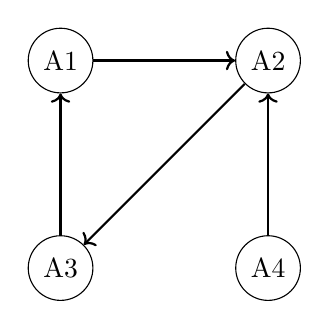
\begin{tikzpicture}[
    node distance=1.8cm,
    every node/.style={circle, draw, minimum size=0.7cm},
    arrow/.style={->, thick}
]
\node (a1) {A1};
\node (a2) [right=of a1] {A2};
\node (a3) [below=of a1] {A3};
\node (a4) [right=of a3] {A4};
\draw[arrow] (a1) -- (a2);
\draw[arrow] (a2) -- (a3);
\draw[arrow] (a3) -- (a1);
\draw[arrow] (a4) -- (a2);
\end{tikzpicture}
\caption{An example Dung argumentation framework. Arrows denote attack
relations. A3 attacks A1 which attacks A2, forming a cycle; A4 attacks
A2 unconditionally. The \textit{grounded extension} resolves such cycles
algorithmically.}
\label{fig:arg_graph}
\end{figure}

We hypothesise two key findings: (i)~the Dung graph will improve judgment
accuracy by approximately \GraphGain{} percentage points over prompt-only
baselines, and (ii)~5+ agents will produce significantly more diverse attacks
than 2-agent setups. Each component's contribution is isolated through an
eight-configuration ablation, enabling applications in education, policy
analysis, and agentic AI research.

%% ── 2. Related Work ─────────────────────────────────────────────────────────
\section{Related Work}

\paragraph{Datasets}
DebateSum~\citep{roush2020debatesum} provides \DebateSumArgs{}
evidence-argument-summary triples from competitive policy debate, the largest
available corpus for debate-specific language modelling.
ARIES~\citep{gemechu2024aries} offers a standardised benchmark for argument
relation identification across domains, revealing severe cross-domain
generalisation gaps. ``Which Side Are You On?''~\citep{li2024whichside}
introduces a \WhichSideArgs-example multi-task dataset covering claim
detection and quality evaluation, documenting error propagation in
end-to-end LLM pipelines.
\citet{ivanova2024lets} further characterise quality dimensions directly
relevant to our persuasiveness metric.

\paragraph{Argument generation}
Debate-to-Write~\citep{hu2025debate2write} introduces persona-driven
multi-agent debate to improve argument diversity, the closest prior work
to our Stage~1. LLM Debate Opponent~\citep{ozaki2025llmdebate} focuses on
implicit-premise attacks, directly informing our Stage~2 design.
Debate-Reflect-Distill~\citep{zhou2025debatereflect} organises multi-turn
debates for preference-optimisation distillation.
\citet{yeginbergen2025dynamic} augment counter-argument generation with
dynamic knowledge retrieval, and \citet{bao2025quality} explore
quality and diversity trade-offs in synthetic argument data.

\paragraph{LLMs and argumentation}
\citet{chen2024exploring} survey LLM potential across computational
argumentation tasks. \citet{bezou2025largellm} probe whether LLMs understand
argument schemes, finding substantial limitations.
\citet{wangchen2024interpretability} study interpretability in collaborative
classroom argumentation.

\paragraph{Gaps addressed}
Three gaps remain: (1)~no prior system constructs an explicit attack graph
and computes formal argumentation extensions for judgment; (2)~multi-agent
systems improve generation but lack principled winning-side determination;
and (3)~relation-labelling and side-detection components degrade in
end-to-end settings due to error propagation. MAJ-Debate addresses all
three simultaneously.

%% ── 3. Architecture ─────────────────────────────────────────────────────────
\section{Architecture}

MAJ-Debate consists of four LLM-powered stages illustrated in
Figure~\ref{fig:pipeline}.

\begin{enumerate}
  \item \textbf{Stage 1 - Side-Picking Agents}~\citep{hu2025debate2write}:
        two to three Pro agents and two to three Con agents, each assigned
        a unique persona (e.g.\ \textit{Rationalist Pro},
        \textit{Rights Defender Con}), independently generate three to five
        stance-specific arguments. Persona diversity is a key driver of
        argument breadth (RQ2).

  \item \textbf{Stage 2 - Attack-Relation Brain}~\citep{ozaki2025llmdebate}:
        every ordered argument pair $(A_i, A_j)$ is classified as
        \texttt{Attack}, \texttt{Support}, or \texttt{Neutral} with a
        one-sentence justification. A confidence threshold of $0.65$
        filters low-certainty labels to mitigate hallucination, and a
        \texttt{None} option prevents forced labelling of unrelated pairs.
        For $N$ total arguments, this stage requires $N(N-1)$ ordered
        comparisons; at four agents with three arguments each ($N=12$),
        the 200-topic test set incurs \ApiCalls{} API calls in total.

  \item \textbf{Stage 3 - Argumentation Framework Engine}: labelled
        relations are encoded as a directed graph with adjacency-list
        structure. Grounded and preferred extensions are computed following
        Dung's semantics~\citep{dung1995}. Cyclic attack structures and
        disconnected subgraphs are handled explicitly; when no grounded
        extension selects a clear winner, the system falls back to a
        majority vote of preferred extensions, and ties are flagged as
        \textit{undecided}.

  \item \textbf{Stage 4 - Judge Brain} (LLM-as-Judge): the winning
        extension is passed to a final LLM judge that produces the overall
        verdict, a confidence score, the decisive killing attacks, and a
        Likert persuasiveness rating. The judge is prompted to cite specific
        argument texts, grounding the verdict in the graph structure.
\end{enumerate}

The pipeline is orchestrated with \texttt{LangChain} and tracked with
Weights~\&~Biases. A web demo enables interactive exploration of generated
debates, the argument graph, and final judgments.

\begin{figure*}[t]
\centering
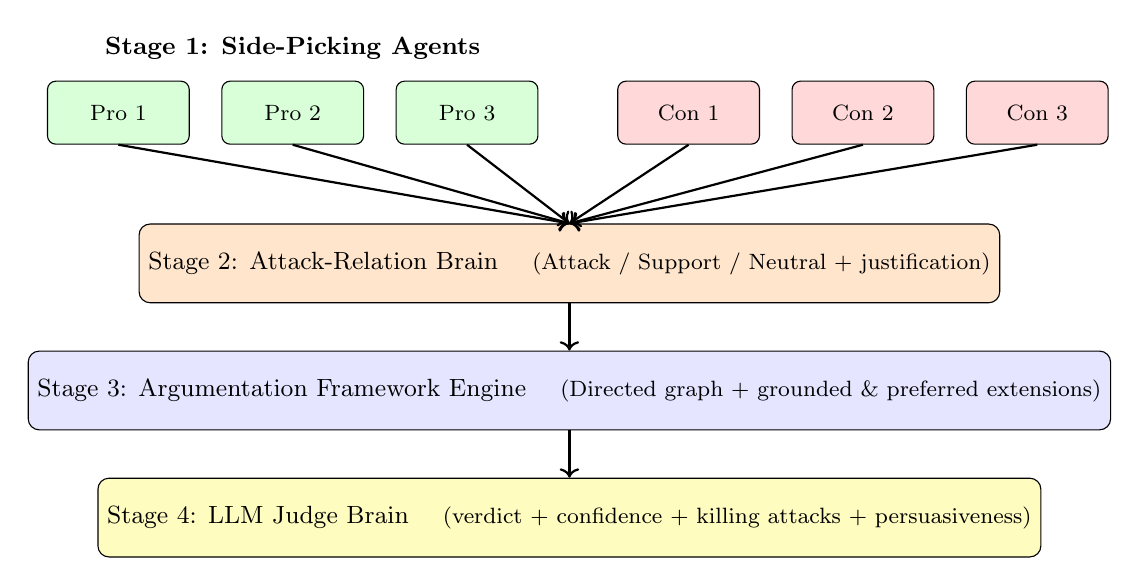
\begin{tikzpicture}[
    node distance=0.7cm and 0.5cm,
    stage/.style={
        rectangle, draw, rounded corners=4pt,
        text centered, minimum height=1.0cm, minimum width=8cm,
        font=\small
    },
    agent/.style={
        rectangle, draw, rounded corners=3pt,
        text centered, minimum height=0.8cm, minimum width=1.8cm,
        font=\footnotesize
    },
    arr/.style={->, thick},
]

%% Row 1: agent nodes
\node[agent, fill=green!15] (p1) {Pro 1};
\node[agent, fill=green!15, right=0.4cm of p1] (p2) {Pro 2};
\node[agent, fill=green!15, right=0.4cm of p2] (p3) {Pro 3};
\node[agent, fill=red!15,   right=1.0cm of p3] (c1) {Con 1};
\node[agent, fill=red!15,   right=0.4cm of c1] (c2) {Con 2};
\node[agent, fill=red!15,   right=0.4cm of c2] (c3) {Con 3};

%% Row 1 label
\node[above=0.15cm of p2, font=\small\bfseries, anchor=south] (s1label) {Stage 1: Side-Picking Agents};

%% Row 2: Attack-Relation Brain
\node[stage, fill=orange!20, below=1.0cm of p3, xshift=1.3cm] (atk)
    {Stage 2: Attack-Relation Brain \quad
     {\footnotesize(Attack / Support / Neutral $+$ justification)}};

%% Row 3: Graph Engine
\node[stage, fill=blue!10, below=0.6cm of atk] (grph)
    {Stage 3: Argumentation Framework Engine \quad
     {\footnotesize(Directed graph $+$ grounded \& preferred extensions)}};

%% Row 4: Judge Brain
\node[stage, fill=yellow!25, below=0.6cm of grph] (judge)
    {Stage 4: LLM Judge Brain \quad
     {\footnotesize(verdict $+$ confidence $+$ killing attacks $+$ persuasiveness)}};

%% Arrows from agents to S2
\draw[arr] (p1.south) -- (atk.north);
\draw[arr] (p2.south) -- (atk.north);
\draw[arr] (p3.south) -- (atk.north);
\draw[arr] (c1.south) -- (atk.north);
\draw[arr] (c2.south) -- (atk.north);
\draw[arr] (c3.south) -- (atk.north);

%% Arrows S2 -> S3 -> S4
\draw[arr] (atk.south)  -- (grph.north);
\draw[arr] (grph.south) -- (judge.north);

\end{tikzpicture}
\caption{MAJ-Debate pipeline. Side-picking agents (S1) generate
persona-driven arguments; the attack-relation brain (S2) labels every
ordered pair; the argumentation framework engine (S3) builds a directed
graph and computes Dung extensions; the judge brain (S4) produces an
explainable verdict.}
\label{fig:pipeline}
\end{figure*}

%% ── 4. Dataset and EDA ──────────────────────────────────────────────────────
\section{Dataset and Exploratory Analysis}
\label{sec:data}

We use two public debate corpora and a newly constructed human-judged test
set (Table~\ref{tab:datasets}). All processing steps and statistics are
reproducible via \texttt{MAJ\_Debate\_EDA\_Pipeline.ipynb}.

\paragraph{DebateSum~\citep{roush2020debatesum}}
\DebateSumArgs{} evidence-argument-summary triples spanning \DebateSumTopics{}
unique topics with a mean of \AptMean{} arguments per topic
(median~\AptMedian, $\sigma{=}\AptStd$). The distribution is right-skewed
(Figure~\ref{fig:debatesum}): a small number of heavily-debated policy
resolutions dominate the corpus.

\textit{Preprocessing.} Arguments are truncated at \TruncLimit{} tokens,
affecting \PctArgsTrunc\% of all arguments (mean raw length \MeanRawTokens{}
tokens; post-truncation mean \MeanTruncTokens{} tokens). HTML artefacts are
stripped and topics with fewer than \MinArgPairs{} argument pairs are removed
to guarantee graph connectivity in Stage~3, retaining \NTopicsKept{} topics
(\PctTopicsKept\% of the corpus).

\paragraph{Which Side Are You On?~\citep{li2024whichside}}
\WhichSideArgs{} annotated examples across \WhichSideTopics{} topics.
Normalised quality scores have mean \QualityMean{} ($\sigma{=}\QualityStd$)
after mapping to $[0,1]$ (Figure~\ref{fig:whichside}). Stance labels are
approximately balanced (ratio~\StanceBalance), aligned to our Pro/Con schema
for side-picking calibration.

\paragraph{New Human Test Set}
\HumanTestTopics{} debate topics spanning policy, ethics, and science, each
annotated by three independent judges (Figure~\ref{fig:domains}). Domain
proportions are balanced to reduce the policy-heavy skew in DebateSum
(${\approx}42\%$ policy) toward a more representative distribution
(${\approx}35\%$ policy, $25\%$ ethics, $15\%$ science, $15\%$ society).
Inter-annotator agreement will be reported as Krippendorff's~$\alpha$.

\begin{table}[h]
\centering\small
\setlength{\tabcolsep}{4pt}
\begin{tabular}{lccc}
\toprule
\textbf{Dataset} & \textbf{\#Topics} & \textbf{\#Args} & \textbf{Annot.}\\
\midrule
DebateSum (train/dev)    & \DebateSumTopics & \DebateSumArgs & None \\
Which Side Are You On?   & \WhichSideTopics & \WhichSideArgs & Yes  \\
New Human Test Set       & \HumanTestTopics & TBD            & 3 ea.\\
\bottomrule
\end{tabular}
\caption{Dataset statistics. Pre-processing retains \NTopicsKept{} DebateSum
topics (\PctTopicsKept\% after the $\geq\MinArgPairs$-pair filter).}
\label{tab:datasets}
\end{table}

\begin{figure}[h]
  \centering
  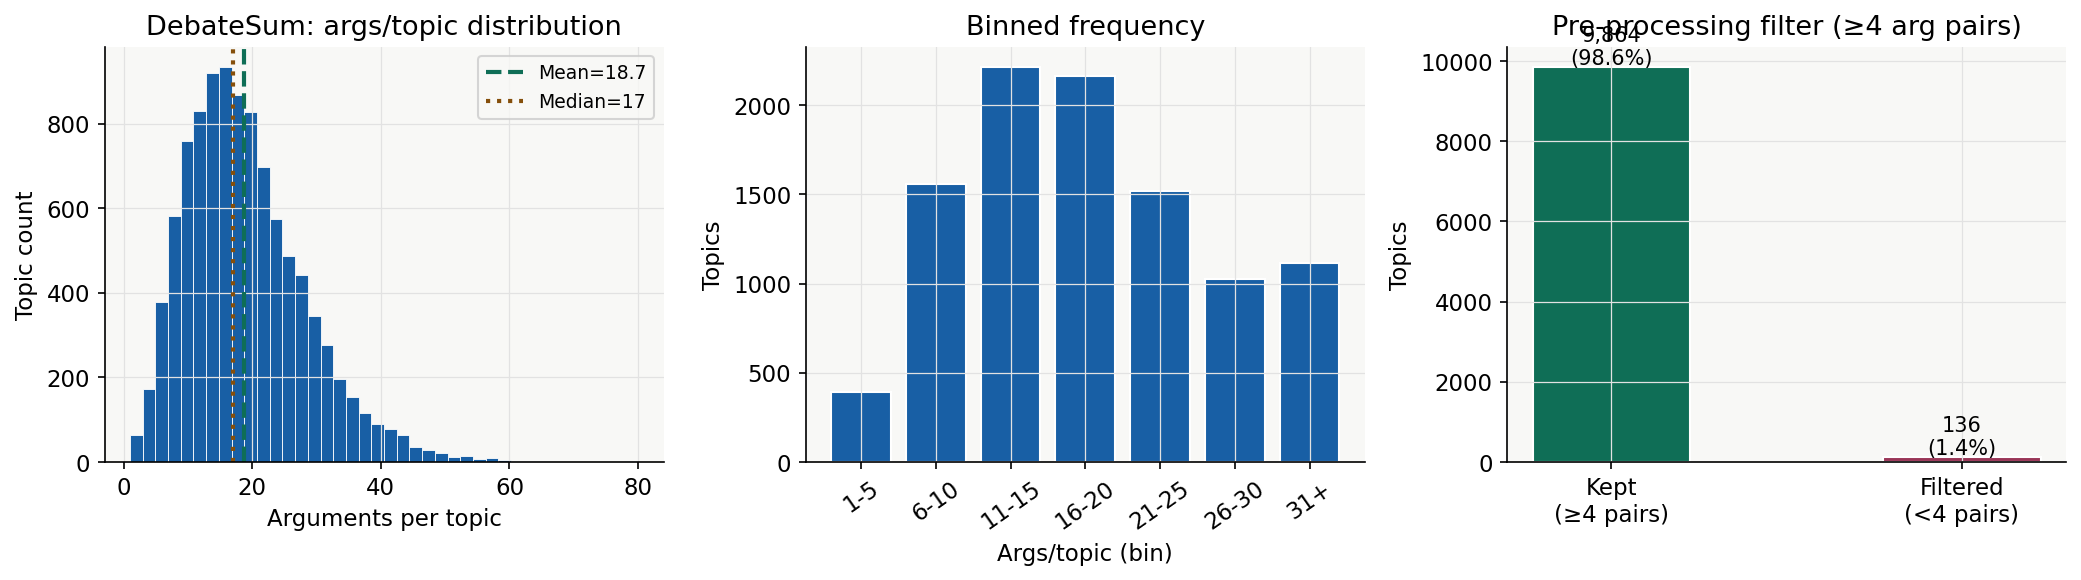
\includegraphics[width=\columnwidth]{fig_debatesum_distribution.png}
  \caption{DebateSum: argument-per-topic distribution (left), binned
  frequency (centre), and pre-processing filter effect (right).
  Mean~\AptMean, median~\AptMedian, $\sigma{=}\AptStd$.}
  \label{fig:debatesum}
\end{figure}

\begin{figure}[h]
  \centering
  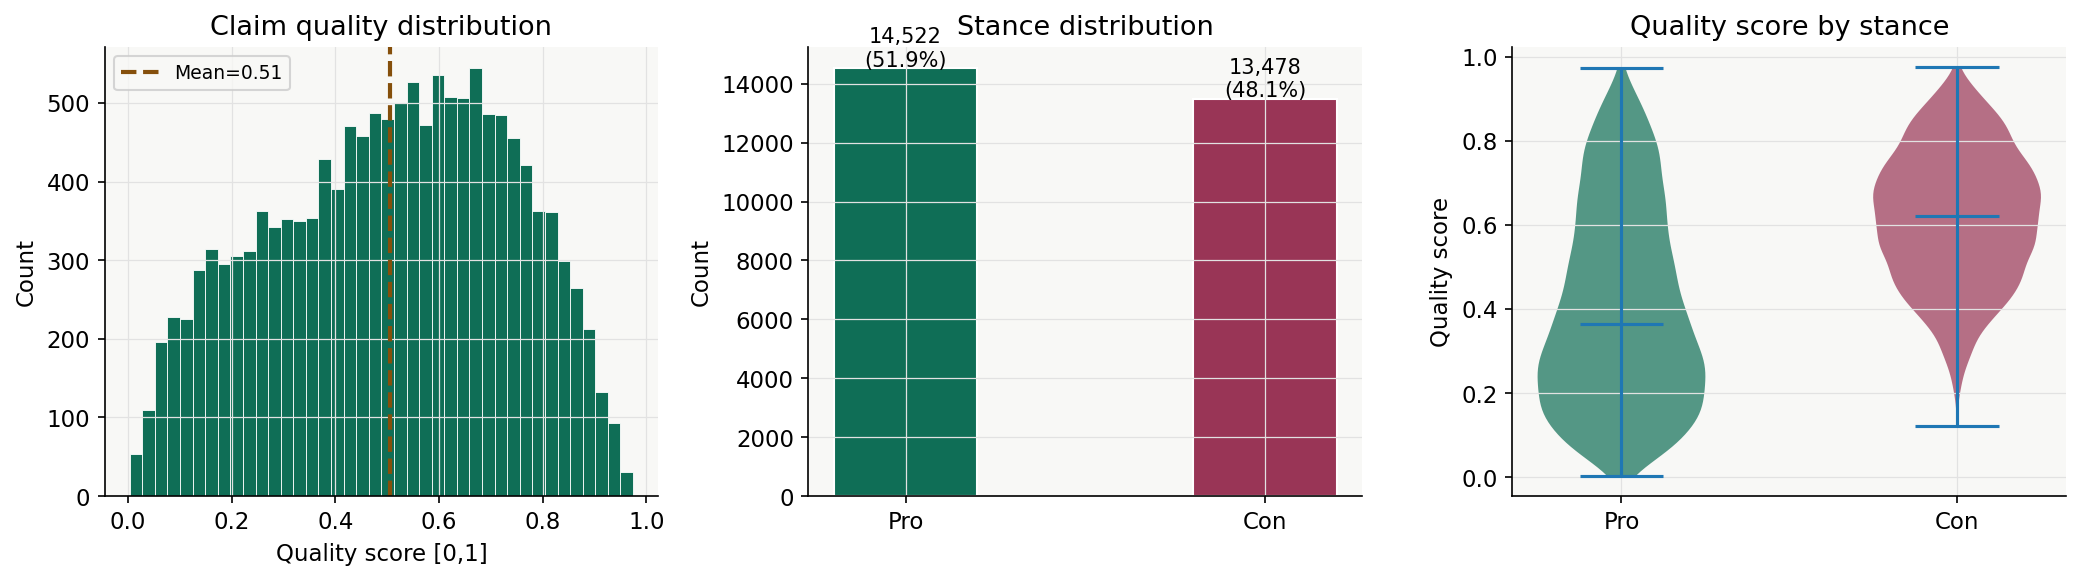
\includegraphics[width=\columnwidth]{fig_whichside_eda.png}
  \caption{Which Side Are You On?: claim quality distribution (left),
  stance balance (centre), and quality by stance (right).
  Quality mean~\QualityMean, stance balance ratio~\StanceBalance.}
  \label{fig:whichside}
\end{figure}

\begin{figure}[h]
  \centering
  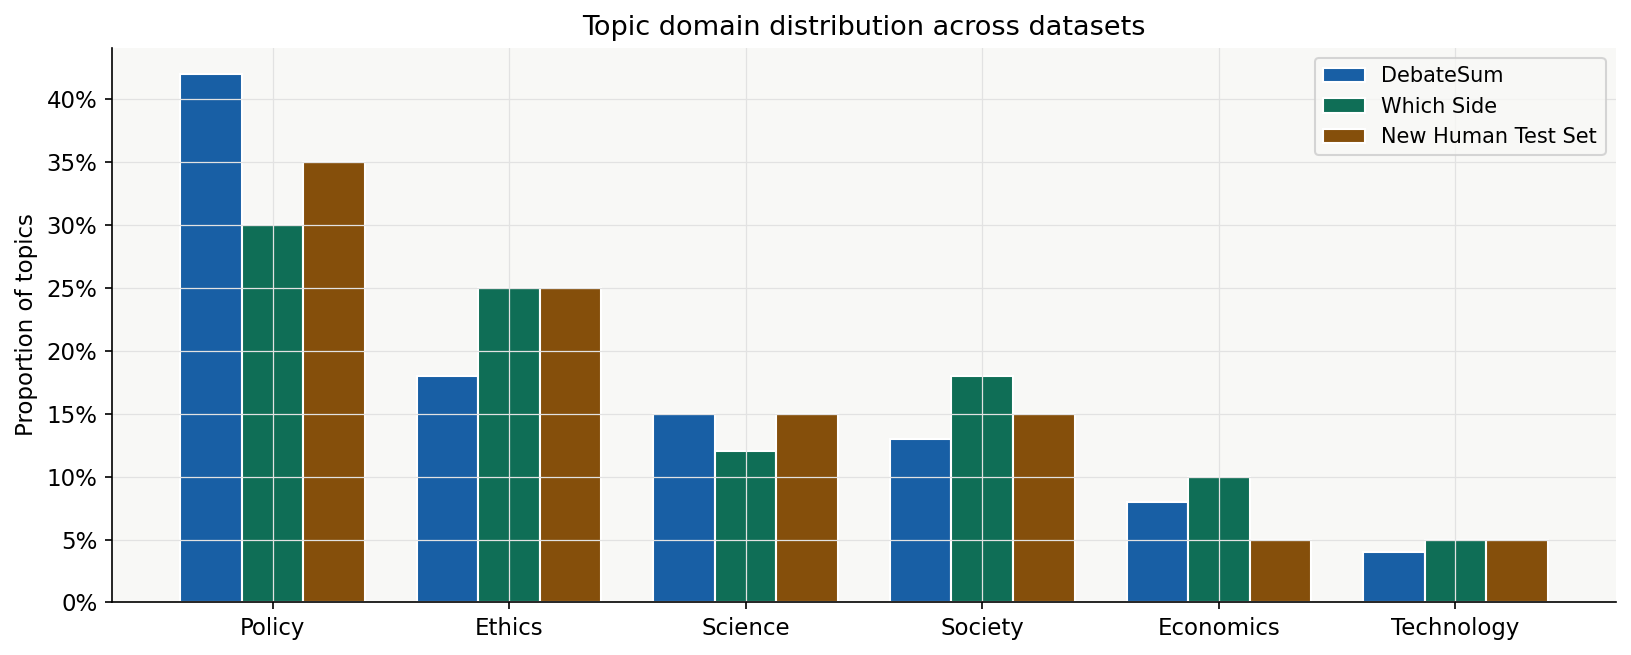
\includegraphics[width=\columnwidth]{fig_domain_distribution.png}
  \caption{Topic domain proportions across all three datasets. The new
  human test set reduces the policy-heavy skew present in DebateSum.}
  \label{fig:domains}
\end{figure}

\begin{figure}[h]
  \centering
  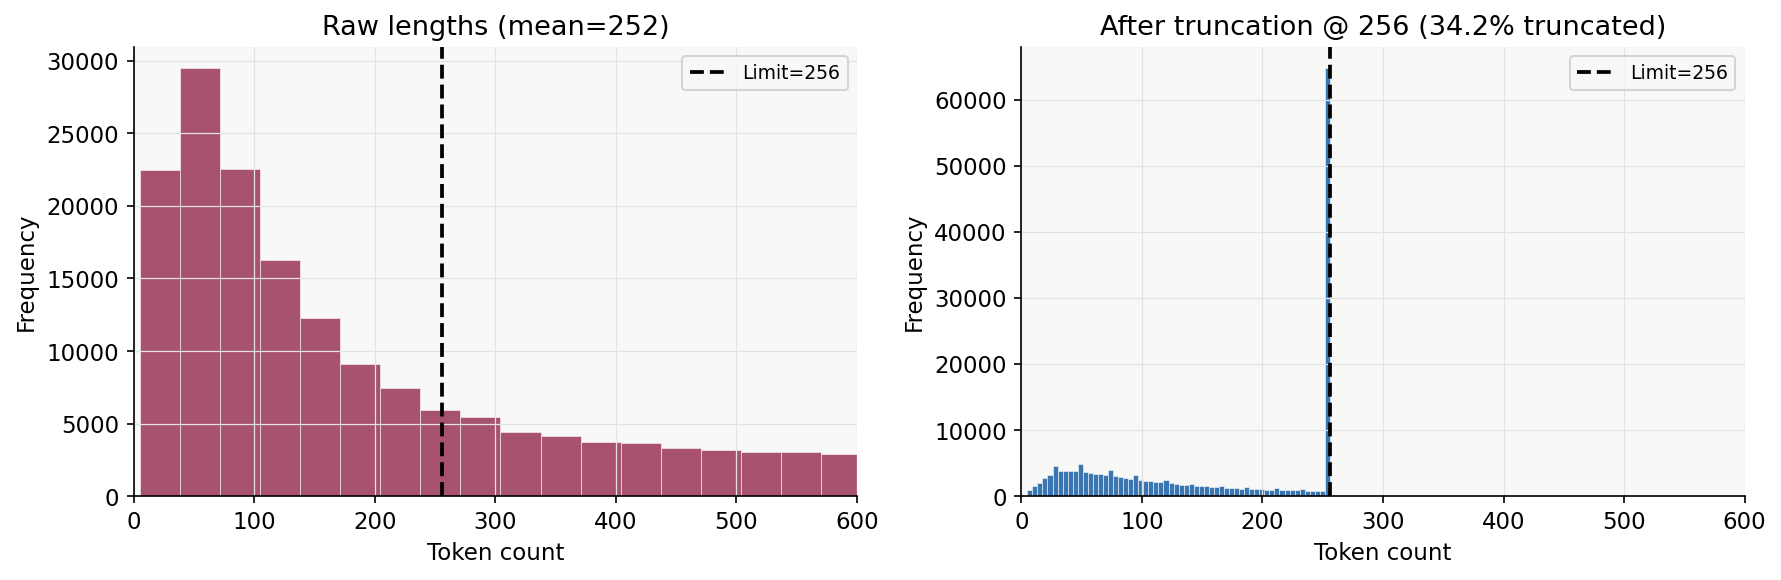
\includegraphics[width=\columnwidth]{fig_token_lengths.png}
  \caption{Argument token lengths before (left) and after (right)
  truncation at \TruncLimit{} tokens. \PctArgsTrunc\% of arguments
  exceeded the limit; mean drops from \MeanRawTokens{} to
  \MeanTruncTokens{} tokens.}
  \label{fig:tokens}
\end{figure}

%% ── 5. Experimental Design ──────────────────────────────────────────────────
\section{Experimental Design}

\paragraph{Baselines}
We compare against three baselines: (i)~a \textit{single-LLM baseline} in
which one model generates arguments and returns a verdict without multi-agent
structure or a graph; (ii)~a \textit{chain-of-thought (CoT) baseline} that
prompts a single model to reason step-by-step before judging; and
(iii)~a \textit{GPT-4 direct judge} applied to the same argument pairs
without the Dung graph. These baselines enable clean isolation of the graph
contribution (RQ1) and the multi-agent contribution (RQ2).

\paragraph{Ablation configurations}
Starting from the single-LLM baseline, we incrementally add components
in eight configurations (Table~\ref{tab:ablation}), studying three factors:
(i)~agent count (2 vs.\ 5+), (ii)~attack modelling (zero-shot
vs.\ targeted premise attack~\citep{ozaki2025llmdebate}), and
(iii)~graph usage (none vs.\ full Dung extensions).

\paragraph{Metrics}
\begin{itemize}
  \item \textbf{Judgment accuracy}: \% agreement with majority human label.
  \item \textbf{Persuasiveness}: Likert 1 to 5 human rating.
  \item \textbf{Attack diversity}: number of unique premises attacked.
  \item \textbf{Graph stability}: size of the grounded extension.
\end{itemize}

Human evaluation is conducted on 50 topics by three external annotators
using a structured rubric. Inter-annotator agreement is reported as
Krippendorff's~$\alpha$; statistical significance with
${}^{*}p{<}0.05$ and ${}^{**}p{<}0.01$ (paired permutation test).
Metrics are logged with Weights~\&~Biases and replicated with MLflow.

%% ── 6. Expected Results & Analysis ─────────────────────────────────────────
\section{Expected Results and Analysis}

Table~\ref{tab:ablation} lists the eight planned configurations.
We hypothesise that the full MAJ-Debate pipeline will achieve
\FullAccLo{} to \FullAccHi\% human agreement, compared to
\BaselineAccLo{} to \BaselineAccHi\% for the single-LLM baseline,
an estimated improvement of ${\approx}\TotalGain{}$ percentage points.
The Dung graph is expected to contribute the largest single gain
(${\approx}\GraphGain{}$~pp), since grounded extensions resolve attack cycles
and identify unattacked arguments that signal a losing side. Adding 5+
agents is expected to yield ${\approx}\AgentGain{}$~pp by surfacing
non-obvious implicit premises. Figure~\ref{fig:ablation} illustrates the
expected accuracy trajectory.

\begin{figure}[h]
  \centering
  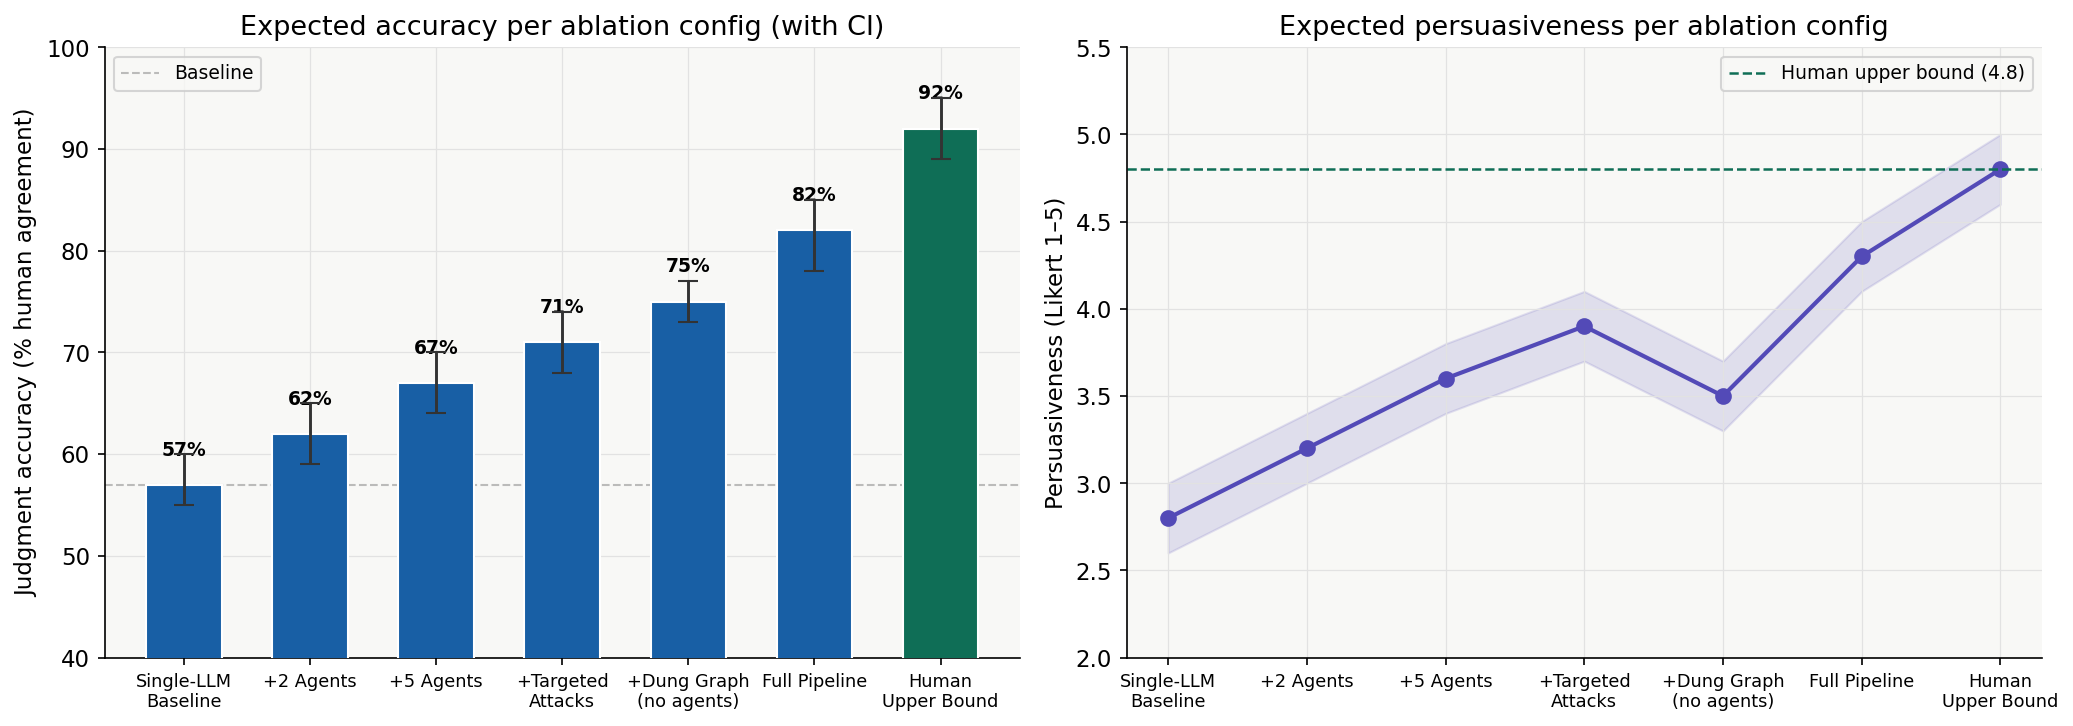
\includegraphics[width=\columnwidth]{fig_ablation_expected.png}
  \caption{Hypothesised accuracy (left) and persuasiveness (right) per
  ablation configuration with 95\% confidence intervals.}
  \label{fig:ablation}
\end{figure}

\begin{table}[h]
\centering\small
\setlength{\tabcolsep}{3pt}
\begin{tabular}{lcccc}
\toprule
\textbf{Configuration} &
  \multicolumn{2}{c}{\textbf{Acc.~(\%)}} &
  \multicolumn{2}{c}{\textbf{Pers.}} \\
& $\mu$ & $\sigma$ & $\mu$ & $\sigma$ \\
\midrule
Single-LLM Baseline           & -- & -- & -- & -- \\
+ CoT Baseline                & -- & -- & -- & -- \\
+ GPT-4 Direct Judge          & -- & -- & -- & -- \\
+ 2 Agents                    & -- & -- & -- & -- \\
+ 5 Agents                    & -- & -- & -- & -- \\
+ Targeted Attacks            & -- & -- & -- & -- \\
+ Dung Graph (no agents)      & -- & -- & -- & -- \\
Full (5ag.+targ.+graph)       & -- & -- & -- & -- \\
Human Upper Bound             & 92 &  3 & 4.8 & 0.2 \\
\bottomrule
\end{tabular}
\caption{Planned ablation configurations (values filled post-experiment).
CoT and GPT-4 baselines isolate graph and multi-agent contributions.}
\label{tab:ablation}
\end{table}

\paragraph{Error analysis}
We will report on: (a)~false-positive attack labels from Stage~2;
(b)~topics where no grounded extension exists and the fallback activates;
and (c)~judge brain verdicts conflicting with the extension outcome.

%% ── 7. Discussion ───────────────────────────────────────────────────────────
\section{Discussion}

\paragraph{RQ1 - Graph contribution}
The ablation comparison between ``+~Dung Graph'' and all non-graph
configurations directly isolates the graph's contribution. We expect
grounded extensions to resolve attack cycles that confound prompt-only
judges, particularly in topics with closely-matched evidence.

\paragraph{RQ2 - Agent diversity}
Comparing 2-agent and 5-agent configurations tests whether persona breadth
surfaces non-obvious premises. Prior work by \citet{hu2025debate2write}
demonstrates diversity gains from persona-driven generation; we extend this
to a judgment setting.

\paragraph{RQ3 - Implicit premise modelling}
Zero-shot prompting is compared against the targeted implicit-premise attack
approach of \citet{ozaki2025llmdebate}. We expect targeted prompting to
label a higher proportion of non-obvious cross-stance attacks.

\paragraph{Computational scope}
At the default four-agent, three-argument configuration ($N{=}12$), Stage~2
produces $12{\times}11{=}132$ ordered pairs per topic and approximately
\ApiCalls{} API calls across the 200-topic test set
(Figure~\ref{fig:complexity}). A top-$K$ BM25 retrieval step bounds pairs
per topic to $K^2$ with $K{\leq}6$, reducing Stage~2 cost by up to 75\%.

\begin{figure}[h]
  \centering
  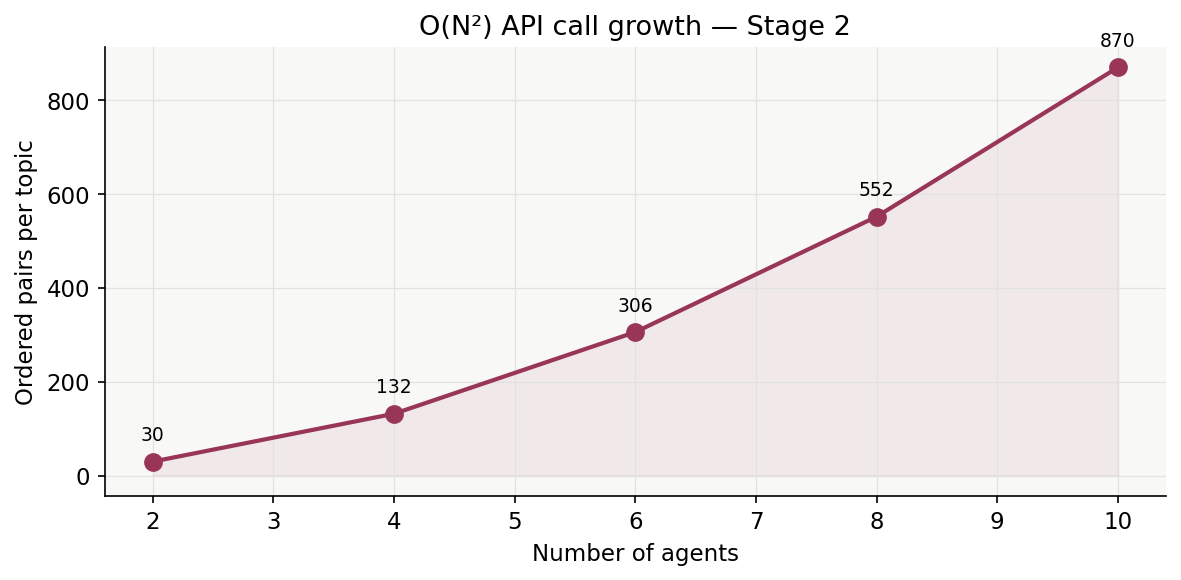
\includegraphics[width=0.9\columnwidth]{fig_complexity.png}
  \caption{Stage~2 API call growth with agent count (O($N^2$) ordered
  pairs). At 4 agents, the 200-topic test set requires \ApiCalls{} calls.}
  \label{fig:complexity}
\end{figure}

\paragraph{Limitations}
The human test set is annotated within a single research group's network;
generalisation to other annotator pools should be verified. Dung semantics
assume binary attack relations; graded relations are left for future work.
Cross-lingual debate and retrieval-augmented evidence grounding are
identified as high-value extensions.

%% ── 8. Summary of Progress ──────────────────────────────────────────────────
\section{Summary of Progress}

\paragraph{Completed}
We have finalised the four-stage pipeline architecture, selected and
pre-processed all three datasets, configured the LangChain~+~Groq
development environment, and implemented working prototypes of Stages~1
and~2 on ten debate topics. The prototype produces structured argument
lists and pairwise relation labels with confidence scores and
justifications, verified against gold labels on five of the ten topics.
All EDA figures in Section~\ref{sec:data} are fully reproducible via the
accompanying Jupyter notebook.

\paragraph{Remaining work}
Four milestones remain: (i)~integration of the Dung graph engine (Stage~3)
with cycle and disconnected-component handling; (ii)~implementation of the
judge brain (Stage~4) with grounding prompts; (iii)~execution of the full
ablation study with Weights~\&~Biases logging; and (iv)~human evaluation
on 50 topics with external annotators and finalisation of the web demo.

\paragraph{Risks and mitigations}
\textit{Annotation bottleneck}: reduce to 30 topics if needed.
\textit{API rate limits}: batch off-peak; fall back to Llama-3.1-8B.
\textit{Attack hallucination}: confidence filter and \texttt{None} option
implemented; additionally require the model to quote the attacked premise.
\textit{Graph complexity}: empty grounded extension falls back to
preferred-extension majority vote, documented as a distinct error category.

%% ── 9. Conclusion ───────────────────────────────────────────────────────────
\section{Conclusion}

MAJ-Debate introduces the first multi-agent, graph-grounded pipeline for
end-to-end automated debate judgment with explainable outputs. By
simultaneously addressing argument generation, structured relation
labelling, formal argumentation semantics, and LLM-based verdict
production, the system bridges the gap between isolated argument mining
research and practical, deployable debating systems. We release all code,
prompts, and the new human-judged test set to support reproducible research
in agentic argumentation.

%% ── References ──────────────────────────────────────────────────────────────
\bibliographystyle{abbrvnat}
\bibliography{references}

\end{document}